\chapter{Поисковые методы идентификации}

\section{Методы поиска}

\subsection{Априорная и текущая информация}

Без априорной информации невозможно построение
работоспособной системы идентификации. Основные
априорные величины определяются на этапе постановки
задачи идентификации. В первую очередь это
параметры масштаба: допустимый диапазон
изменения параметров \( \mathbf{P}\),
характерное время работы
идентифицируемой системы, а также
требуемая точность и скорость идентификации
(могут быть заданы различными способами).
В этот список может входить и максимальная скорость изменения параметра.
В процессе работы эти параметры могут уточнятся по текущей информации.

Следующую часть априорной (по отношению к идентификации) информации
предоставляет процесс синтеза критерия идентификации.
В первую очередь, это сам вид критерия. Им определятся
как диапазон изменения величины этого критерия, так и
динамические свойства: характерное/минимально время
оценивали \(\tau\) (или даже оценка зависимости $\tau$ от точности и других параметров),
характерное время реакции системы на изменение
параметра с учётом динамики измерения \(q\).




\subsection{Основные параметры поиска}

xxx

\subsection{ Использование множества моделей / агентов}

Введём необходимые для дальнейшегго изложения определения.

Определение: \textbf{поисковый агент} -- это динамическая система, получающая выходной ($x(t)$),
и, при необходимости входной сигнал ($u(t)$) от одной или нескольких моделей,
может быть информацию от других поисковых агентов,
на основании значения критерия идентификации
реализующая алгоритм настройки параметра модели (моделей)
таким образом, чтобы обеспечить идентификацию заданного параметра.

Один поисковый агент может управлять как одной моделью (рис.~\ref{atu:f:agent1}),
так и несколькими.
При этом он может использовать информацию,
как полученную непосредственно от других агентов,
так и вычисленную в результате обработки данных на других уровнях системы идентификации.

\begin{figure}[htb!]
\begin{center}
% vi:syntax=tex
\begin{tikzpicture}
  \bXStyleBloc{semiboldline,inner sep=2pt};
  \bXLineStyle{medline};
  % --- U
  \bXInput{U};
  % --- M
  \bXBlocL[2.0]{M}{$\mathbf{M}_i$}{U};
  \bXLink[$u(t)$]{U}{M};
  % --- Q
  \bXBloc[3.5]{Q}{$q(t)$}{M};
  \path (Q.east) ++(0.0,-1.0em) coordinate (Qqm);
  \path (Q.south west) ++(-0.3,-0.4) coordinate (BLKlb);
  \bXLink[$x_i(t)$]{M}{Q};
  % --- F
  \bXBloc[2.5]{F}{$F(q_o,q_{mi})$}{Q};
  \path (F.west) ++(0.0,-1.0em) coordinate (Fqm);
  \path (F.west) ++(0.0,+1.0em) coordinate (Fqo);
  \path (Fqo) ++(-1.6em,+2.8em) coordinate (Fqoi) {};  % external input
  \draw[medlinep] (Fqoi) |- (Fqo);
  \node[below right] at (Fqoi) {$q_o(t)$};
  \bXLink[$q_i(t)$]{Qqm}{Fqm};
  % --- P
  \bXBloc[2]{P}{$P$}{F};
  \draw[boldline,<->] (P.north) -- +(0,0.8);
  \path (P.north east) ++(0.1,+0.4) node (BLKrt) {};
  \bXLink[$F_i(t)$]{F}{P};
  % -- output
  \bXOutput[2.8]{Po}{P};
  \bXLink[$p_i(t)$]{P}{Po};
  \bXOutput[1.0]{Por}{P};
  \fill(Por) circle[radius=0.05];
  \bXLineStyle{semiboldline};
  \bXReturn{Por}{M}{$p_i(t)$};
  % -- block
  \draw[subelem] (BLKlb) |- (BLKrt) |- (BLKlb);
  \bXStyleBlocDefault;
  \bXDefaultLineStyle;
  %
  \TikzAddPadding
  %
\end{tikzpicture}

\end{center}
\caption{Поисковый агент, настраивающий параметр одной модели}
\label{atu:f:agent1}
\end{figure}


В случае, когда один агент настраивает несколько моделей,
или/и, если пространство параметров имеет размерность больше единицы,
вместо простого индекса $i$ могут применяется составные.

В простейших случаях возможно построение системы идентификации
с одной моделью и, соответственно, одним поисковым агентом.
Примерами такого похода могут служить
метод синхронного детектора \cite{adopt_cont_sys}
и оригинальный адаптивно-поисковый метод \cite{mich_92}.
Применение одномодельных методов требует определённого механизма
сохранения истории процесса поиска, по крайней мере в пределах
одного поискового ``периода''. Это сильно ограничивает диапазон
применимости данных методов, в первую очередь -- из-за значительных
временных затрат на повторяющийся поиск.

Применение пары моделей \cite{atu_asau3}
(в этом случае имеет смысл говорить об одном поисковом агенте)
позволяет с меньшими временными затратами оценить градиент функции качества,
и, как следствие -- определить значение параметра. Также значительным плюсом
такого подхода является меньшая скорость изменения параметров моделей.

Тем не менее, при использовании пары моделей неоправданно много времени
тратится на перемещение поисковой пары, особенно при резких изменениях
идентифицируемого параметра. Поэтому, использование множества
поисковых агентов может кардинально уменьшить время идентификации.

Каждый поисковый агент, определяя величину $q_{i}(t)$ , и получая $q_o(t)$,
вычисляет безразмерную функцию качества идентификации
$F(q_o,q_i)$.

С учётом обозначения
%
\[
  q_r = \frac{q_o - q_m}{q_\gamma},
\]
%
\noindent
представлены наиболее распространённые виды таких функций~\cite{atu_ISDMCI2016}:
%
\begin{equation}
  F_{\mathrm{gauss}} = \exp( - q_r^2 ),
\label{atu:eq:F_gauss}
\end{equation}
%
\begin{equation}
  F_{\mathrm{parabolic}} = 1 - q_r^2 \left( 1 - \frac{1}{e} \right),
\label{atu:eq:F_parabolic}
\end{equation}
%
\begin{equation}
  F_{\mathrm{triangle}} = 1 - |q_r| \left( 1 - \frac{1}{e} \right),
\label{atu:eq:F_triangle}
\end{equation}
%
\begin{equation}
  F_{\mathrm{hyper}} = \frac{1}{ 1 + |q_r| \left( 1 - \frac{1}{e} \right)},
\label{atu:eq:F_hyper}
\end{equation}
%
\begin{equation}
  F_{\mathrm{log}} = 1 - \ln \left( 1 + |q_r| \right) \frac{1-1/e}{\ln(2)}.
\label{atu:eq:F_log}
\end{equation}

Для всех рассмотренных функций $q_\gamma$ -- величина, обратная чувствительности
функции качества, задаёт масштаб и рабочий диапазон функции качества (рис.~\ref{atu:f:F_types}).
При этом, при необходимости, значения этих функций могут быть искусственно ограничены диапазоном $[0;1]$.
Каждая имеет свой набор преимуществ и недостатков~\cite{atu_ISDMCI2016}.

\begin{figure}[htb!]
  \centerline{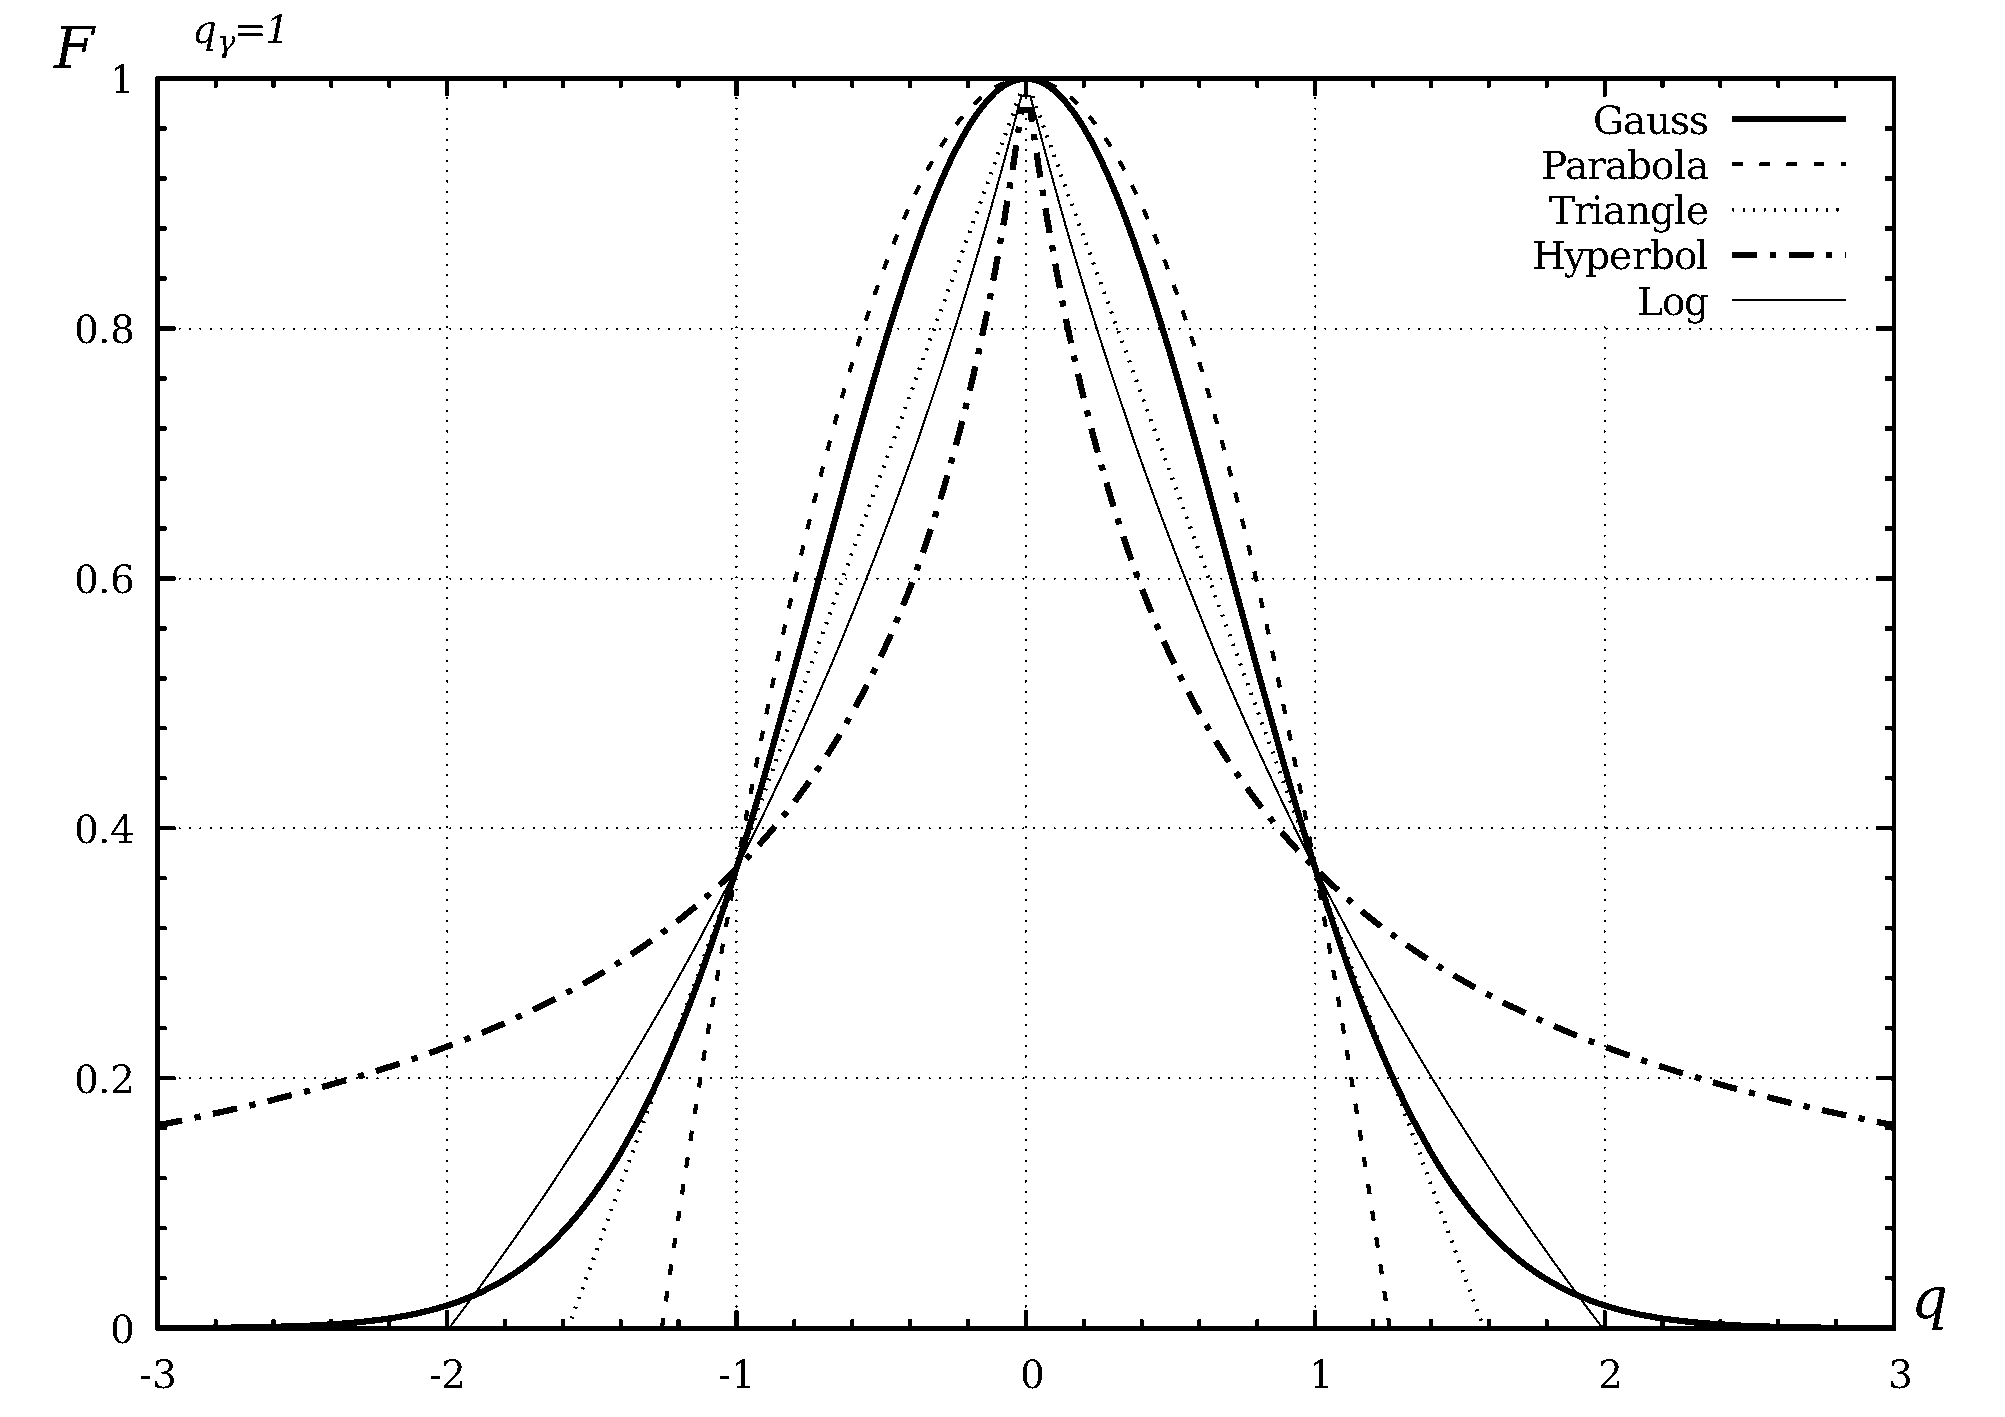
\includegraphics[width=45\TW]{p/F_types.png} }
  \caption{Функции качества идентификации (\ref{atu:eq:F_gauss})--(\ref{atu:eq:F_log})}
  \label{atu:f:F_types}
\end{figure}

Рассмотрим случай, когда каждый агент взаимодействует с двумя своими ближайшими соседями,
запрашивая у них величины $p$ -- текущее значение параметра и $F$.
При анализе конкретного агента, для упрощения записи, его индекс $i$ обозначим как ``c'' (current),
предыдущий получает индекс ``l'' (left), а последующий -- ``r'' (right).
Для единообразия дополним множество моделей двумя неподвижными псевдомоделями (fake models),
обозначив их индексами ``ll'' и ``rr''. Для псевдомоделей считаем $  F_{ll} = F_{rr} = 0$,
а координаты выбираются за пределами рабочего диапазона поиска.


\subsubsection{Один агент}

Единственный неподвижный агент практически не имеет смысла
с точки зрения синтеза системы идентификации.
Он может сигнализировать о том, что в пределах
\(\tau\) модель была или не была достаточно адекватна
объекту.

Наличие истории и возможность перемещаться дают возможность
построить систему идентификации и на одном агенте.
В качестве истории могут использоваться, в том числе,
динамические свойства идентифицируемого объекта
(оригинальный метод АПИ). Также могут быть
применены интегрирующие элементы агента идентификации
(синхронный детектор, \ldots).

\subsubsection{Пара агентов}

Пара агентов, взаимодействующая между собой,
способна оценить градиент функции качества,
и, следовательно, обеспечить смещение в требуемом направлении.

С учетом глобальной информации возможна адаптация параметров пары.
В свою очередь, информация, полученная от пары может
использоваться для уточнения глобальных параметров.

\subsubsection{Триплет агентов}

Три соседних агента, взаимодействующие между собой,
способны не только оценить градиент функции качества в своей окрестности,
но и определить (опять же, оценочно) наличие там максимума.

\paragraph{Идеальный случай}

Пусть зависимость $q(p)$ задана самым простым и благоприятным для идентификации способом:
%
\[
  q(p) = p_0 + b_p p .
\]
Шумы измерения и прочие помехи отсутствуют.
Рассмотрим 3 соседних поисковых агента: $A_l$, $A_c$, $A_r$.
Тогда, если $p_o \in [ p_l, p_r ] $, оценка положения
идентифицируемого параметра $p_e$, выполненная агентом $A_c$,
должна совпадать с реальным значением параметра объекта: $p_e = p_o $.
Если $p_o \notin [ p_l, p_r ] $, то конкретное расположение
$p_e$ значения не имеет, достаточно потребовать определения направления
этого расположения относительно диапазона. % TODO: и может быть чего-то ещё для адаптации


% TODO: full rewrite,
\begin{figure}[htb!]
  \centerline{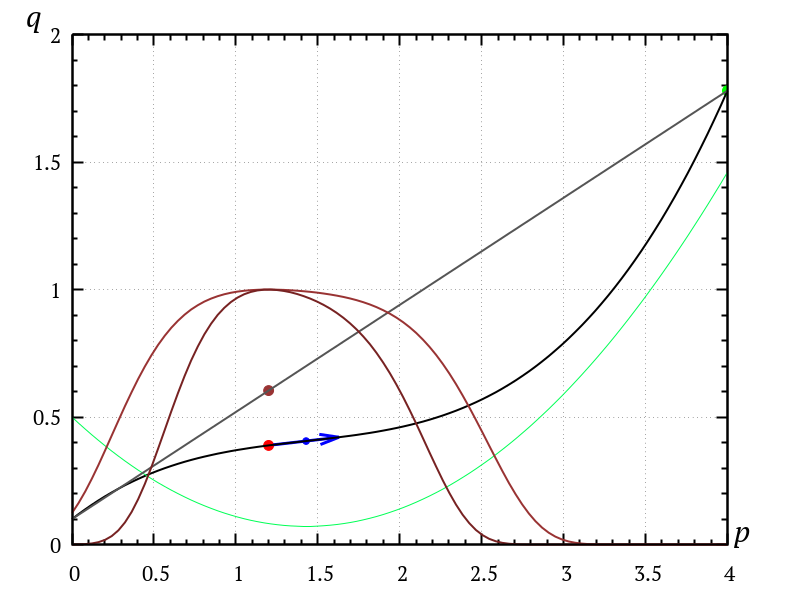
\includegraphics[width=0.6\textwidth]{pq_1x2.png} }
  \caption{ $q(p)$, $F(q(p))$, part1 }
  \label{atu:pq_1x2}
\end{figure}

\begin{figure}[htb!]
  \centerline{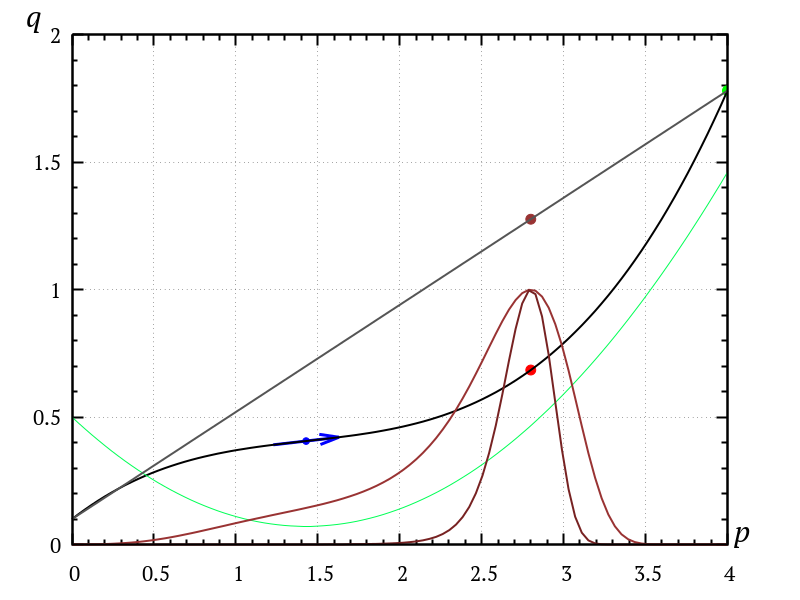
\includegraphics[width=0.6\textwidth]{pq_2x8.png} }
  \caption{$q(p)$, $F(q(p))$, part2 }
  \label{atu:pq_2x8}
\end{figure}

\subsubsection{Ансамбль агентов}

\subsection{Адаптация}

\Cmt{
Какие параметры системы идентификации можно адаптировать
и на каком уровне.

Когда имеет смысл играть с чувствительностью.

Как близко имеет смысл подводить модели к экстремуму?
}

\subsection{Время и история}

Способы учёта истории системы и динамических характеристик.

Явное представление истории -- каждый агент имеет способ хранения и использования
информации о предыдущих значениях параметра и критерия.

Неявное представление истории -- тот факт, что в данный момент времени известно
текущее значение параметра и критерия, с учетом известных значений
параметров поиска самого агента, может нефвно дать ограниченную информацию
о предудущием состоянии.

Стабильные/мобильные модели.

История: локальная + глобальная




Рассмотрим 3 подхода к определению
точки максимума функции качества, а следовательно -- значения идентифицируемого параметра \cite{atu_st99,atu_jacs2015}.
Первый -- реализация
метода COG (Center of gravity, Такаги-Сугено) \cite{atu_asau25,atu_csit2015},
используемого при дефаззификации систем нечёткой логики:
%
\begin{equation}
  p_{ge}
  =
  \frac{\sum\limits_{i=0}^{n-1} F_{i} p_{i}}
       {\sum\limits_{i=0}^{n-1} F_{i} }
  .
  \label{atu:eq:p_ge}
\end{equation}

Второй подход призван уменьшить зависимость первого
от влияния локальных экстремумов и границ. В этом
случае определяется модель $M_{i_{m}}$ с максимальным значением
$F$, а в оценке используется только ближайшая окрестность этой модели:
%
\begin{equation}
  p_{le}
  =
  \frac{ F_{i-1} p_{i_m-1} + F_{i} p_{i_m} + F_{i+1} p_{i+1} }
       { F_{i-1}           + F_{i}         + F_{i+1}         }
  .
  \label{atu:eq:p_le}
\end{equation}

Третий подход отличается от второго тем, что по трём точкам вблизи  $M_{i}$
функция $F(p)$ аппроксимируется параболой, и абсцисса её вершины задаёт искомое
значение параметра. Сместим начало координат в точку
$ ( p_c, F_c ) $. Тогда
%
\[
  \tilde{p}_c = 0, \,
  \tilde{p}_l = p_l - p_c, \,
  \tilde{p}_r = p_r - p_c.
\]
%
\[
  \tilde{F}_c = 0, \,
  \tilde{F}_l = F_l - F_c, \,
  \tilde{F}_r = F_r - F_c.
\]
%
\[
  \left\{
    \begin{array}{l}
      a_2 \tilde{p}_l^2 + a_1 \tilde{p}_l  = \tilde{F}_l
      \\
      a_2 \tilde{p}_r^2 + a_1 \tilde{p}_r  = \tilde{F}_r
    \end{array}
  \right. .
\]
%
\[
  a_1 = \frac{\tilde{F}_r \tilde{p}_l^2 - \tilde{F}_l \tilde{p}_r^2 }
             { \tilde{p}_l^2 \tilde{p}_r  + \tilde{p}_l \tilde{p}_r^2 }.
\]
%
\[
  a_2 = \frac{\tilde{F}_r \tilde{p}_l - \tilde{F}_l \tilde{p}_r }
             { \tilde{p}_l^2 \tilde{p}_r  + \tilde{p}_l \tilde{p}_r^2 }.
\]

\begin{equation}
  \tilde{p}_e = - \frac{a_1}{2 a_2};
  \;
  p_e = p_c -- \frac{a_1}{2 a_2}.
  \label{atu:eq:p_e}
\end{equation}


При этом, если
$ p_e \notin [ p_l, p_r ] $, или $ a_2 \ge 0 $, то значение $p_e$ искусственно
ограничивается этим диапазоном. Значение $p_e$ для модели с индексом
$i_m$ обозначим как $p_{ee}$ и будем считать
текущим значением идентифицируемого параметра, полученным с помощью
третьего подхода. Ошибки идентификации в пространстве параметров
для рассмотренных трёх подходов обозначим соответственно:
%
\begin{equation}
  e_{ge} = p_{ge} - p_o, \;
  e_{le} = p_{le} - p_o, \;
  e_{ee} = p_{ee} - p_o.
  \label{atu:eq:e_xx}
\end{equation}


Динамика изменения параметров моделей (поисковых агентов) задаётся следующим образом:
%
\begin{equation}
  \od{p_c}{t} = v_f f_t(t),
  \label{atu:eq:dp_dt}
\end{equation}
%
\noindent
где $f_t$ -- сумма всех действующих ``сил'', $v_f$ -- коэффициент
пропорциональности. Рассмотрим 3 действующие силы
($ f_t = f_c + f_n + f_e $):

\begin{enumerate}
  \item
    $f_c = -k_c (p_c - p_{c,0}) $ -- ``сила притяжения'' к начальному значению
    параметра
    для данной модели. Наличие этой силы не даёт всем моделям принять одно
    и то же значение параметра вблизи экстремума, и, следовательно,
    прекратить процесс поиска. Это также позволяет быстро переключиться
    на другую модель в случае быстрого изменения параметра объекта.

  \item
    $f_n = k_n ( p_r - 2 p_c + p_l ) $ -- ``сила взаимодействия''
    с соседями. Обеспечивает более равномерное распределение
    параметров моделей вблизи экстремума.

  \item
    $f_e = - k_e ( p_c - p_e ) $ -- ``сила притяжения'' к локальной
    оценке экстремума, определённого по выражению~(\ref{atu:eq:p_e}).

\end{enumerate}

Результаты моделирования показали, что в некоторых случаях
имеет смысл введение дополнительных сил ``барьерного'' вида,
для исключения пересечения траекторий поисковых агентов, или же их ухода из рабочего диапазона.



Для определения как точности, так и скорости работы системы
идентификации, при моделировании процесса идентификации
значения идентифицируемого параметра задавались следующими образами:
%
\begin{equation}
  p_o(t) = p_0 +  U_{p} \sin( \omega_{p} t ),
  \label{atu:eq:p_sin}
\end{equation}
%
\begin{equation}
  p_o(t) = p_0 + U_{p} \sign \sin( \omega_{p} t ).
  \label{atu:eq:p_sign}
\end{equation}

При этом измерялись среднеквадратические ошибки идентификации,
что позволило исследовать применимость систем идентификации
при различной динамике изменения параметров, а также
настроить параметры самой системы идентификации.

Сколько всего надо моделей? Размер пространства параметров.
Рой, коллектив, главнюк.
Зачем агентам перемещаться?


\textbf{ Рой } -- множество агентов, обеспечивающее идентификацию за счёт
сосредоточения максимального количества агентов
в области предполагаемого максимума функции качества.
Обычно -- три составляющие поведения
(движение о оцениваемому локальному экстремуму, -- к глобальному, случайная составляющая).

\Cmt{Для сравнения требуется и это промоделировать.
Достаточно накладно -- надо много агентов.}

Достоинства -- простота алгоритмов.
Недостатки -- требуется избыточное количество агентов.
Значительная часть агентов, находящихся вблизи экстремума,
практически не приносит информации. Роевые
алгоритмы (как и их прообразы в живой природе) ориентированы
для увеличения добычи ресурсов, а не информации.

\textbf{ Ансамбль } -- множество агентов, обеспечивающее идентификацию за счёт
распределения агентов таким образом, который обеспечивает как
точность идентификации за счёт ограниченного скопления агентов
в областях предполагаемых максимумов, так и оперативное переключение
на другие области при изменении параметров за счёт недопущения
неоправданной скученности агентов.

\Cmt{ Заметная часть новизны планируется здесь}



\subsection{Качество идентификации}

Два способа -- по критерию (или функции качества)
или по параметру.

Представляется достаточно очевидным, что
С учётомм того факта, что

\Cmt{Расширить из кандидатской с учётом времени и множества моделей.}

Процесс поисковой идентификации заключается в настройке параметров одной
или нескольких моделей, анализу критериев идентификации
(или соответствующих функций качества), и оцениванию по этой информации
значения идентифицируемого параметра. При использовании в целях идентификации нескольких моделей,
появляются общие действия, применяемые к каждой из них.




\section{Выводы по разделу 3}

Выводы.

